\documentclass[utf8]{../IncArticle}
\graphicspath{{../}}
\usepackage{longtable, bm}

\UDK{004.7}
\title{Пример оформления доклада}

\AddAuthor{Автор1}{И}{мя}{О}{тчество}{}
\AddAuthor{Автор2}{И}{мя}{О}{тчество}{Иркутск}

\date{}
\setcounter{page}{1} % Начало нумерации страниц доклада
\begin{document}

\begin{abstract}
Область исследования. Основная идея доклада. Главные результаты. Объем - от 80 до 250 слов.
\end{abstract}

\begin{abstract}[english]
Annotation in English
\end{abstract}

\introduction
Введение в \term[Проблема]{проблему}:

\begin{itemize}
\item пункт 1 \cite{m1};
\item пункт 2.
\end{itemize}

Некоторые соображения:
\begin{enumerate}
\item первое \cite{m2};
\item второе \cite{m3}.
\end{enumerate}
Объем доклада до 50 страниц.

\section{Некоторые фрагменты оформления доклада}


\begin{definition}[Новое понятие]
Термин и его определение
\end{definition}

\section{Еще один раздел}

\begin{theorem}[Необыкновенная теорема]
Текст теоремы
\end{theorem}

\begin{algorithm}[Поиск фундаментального множества циклов]
Запись алгоритма
\end{algorithm}

\subsection{Запись формул}
Используйте стандартные средства отображения формул.

Отдельное уравнение.

\begin{equation}%(7)
2l = \bm{q}_{L}{'}\bm{e} = \bm{e}{'}\textbf{Г}_{L}\bm{e}\Leftarrow\bm{q}_{L}\equiv\textbf{Г}_{L}\bm{e};
\end{equation}

Очень длинное уравнение.


\begin{equation}%(13)
\begin{split}
\bm{u}_0 = \bm{Y}^{-1}\bm{j}&\rightarrow\bm{i}_0 = \bm{Y}_0\bm{u}_0 = \bm{Y}_0\bm{Y}^{-1}\bm{j}\\
      &\rightarrow\bm{u}_1 = -\bm{K}{'}\bm{u}_0 = -\bm{K}{'}\bm{Y}^{-1}\bm{j}\
      \rightarrow\bm{i}_1 = \bm{Y}_1\bm{u}_1 = -\bm{Y}_1\bm{K}{'}\bm{Y}^{-1}\bm{j};
\end{split}
\end{equation}

Группа уравнений.

\begin{subequations}
\begin{eqnarray}%19
\bm{Yu}_0 &=& \bm{j} - \bm{KY}_1\varepsilon,\Leftarrow\bm{Y}\equiv\bm{Y}_0 + \bm{KY}_1\bm{K}{'},			\\
\bm{Ri}_1 &=& \varepsilon - \bm{K}{'}\bm{R}_0\bm{j},\Leftarrow\bm{R}\equiv\bm{R}_1 + \bm{K}{'}\bm{R}_0\bm{K}.
\end{eqnarray}
\end{subequations}

\subsection{Таблицы}
\begin{table}[h]
	\centering\small
\caption{Сравнение видов абстрактной живописи\label{tab1}}
\begin{tabular}{|c|p{35mm}|c|c|c|c|c|c|c|c|c|}\hline\hline
№	&{\bf Вид живописи} &\multicolumn{5}{|c|}{\bf Артефакт}&\multicolumn{2}{c|}{\bf Творец}&\multicolumn{2}{c|}{\bf Зритель}\\\hline
1	&  Импровизация &&&&&&&&& \\%\hline
  & - результат & +	&   & + &    &  & + &   & +	& \\
  & - процесс	  &   & + & + & \# &  & + &   & + & \\
\hline
2	& Фрактальная	& +	& \#&	+	&		 &  &   &	\#&	+ &	\\
\hline
3	& Геометрическая&	+	&   &	+	&	   &	& +	& \#&	+	& \\
\hline
4	& Авангард	    & +	&	  & +	&    &  &	+	&   & +	& \\
\hline
5	& Космос	      & +	&   &	+	& \# &	&   &	+	& +	&\\
\hline
6	& Динамическая	&	  & +	&	  & +	 &  &	\#&	+	& +	&\\
\hline
7	& Либернетическая&	&	+	&\#	& +	 &+	& +	&+&		&+ \\
\hline
	&                &М	&П	&С	&Д	&Р	&Л	&К	&Па	&Ак\\
\hline\hline
\end{tabular}
\end{table}

Можно использовать окружение {\sf longtable}.

\subsection{Рисунки}
Схемы лучше рисовать в Microsoft Visio и затем преобразовывать в формат PNG или JPG (300 dpi).

\begin{figure}[h]
\begin{center}\small
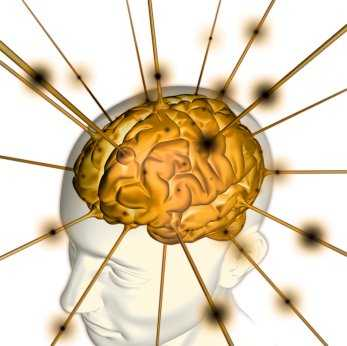
\includegraphics [height=40mm]{pics/mindpowerneg.jpg}%width=100mm
\caption{Образ инкогнито\label{fig1}}
\end{center}
\end{figure}

\begin{figure}[ht]
\begin{center}\small
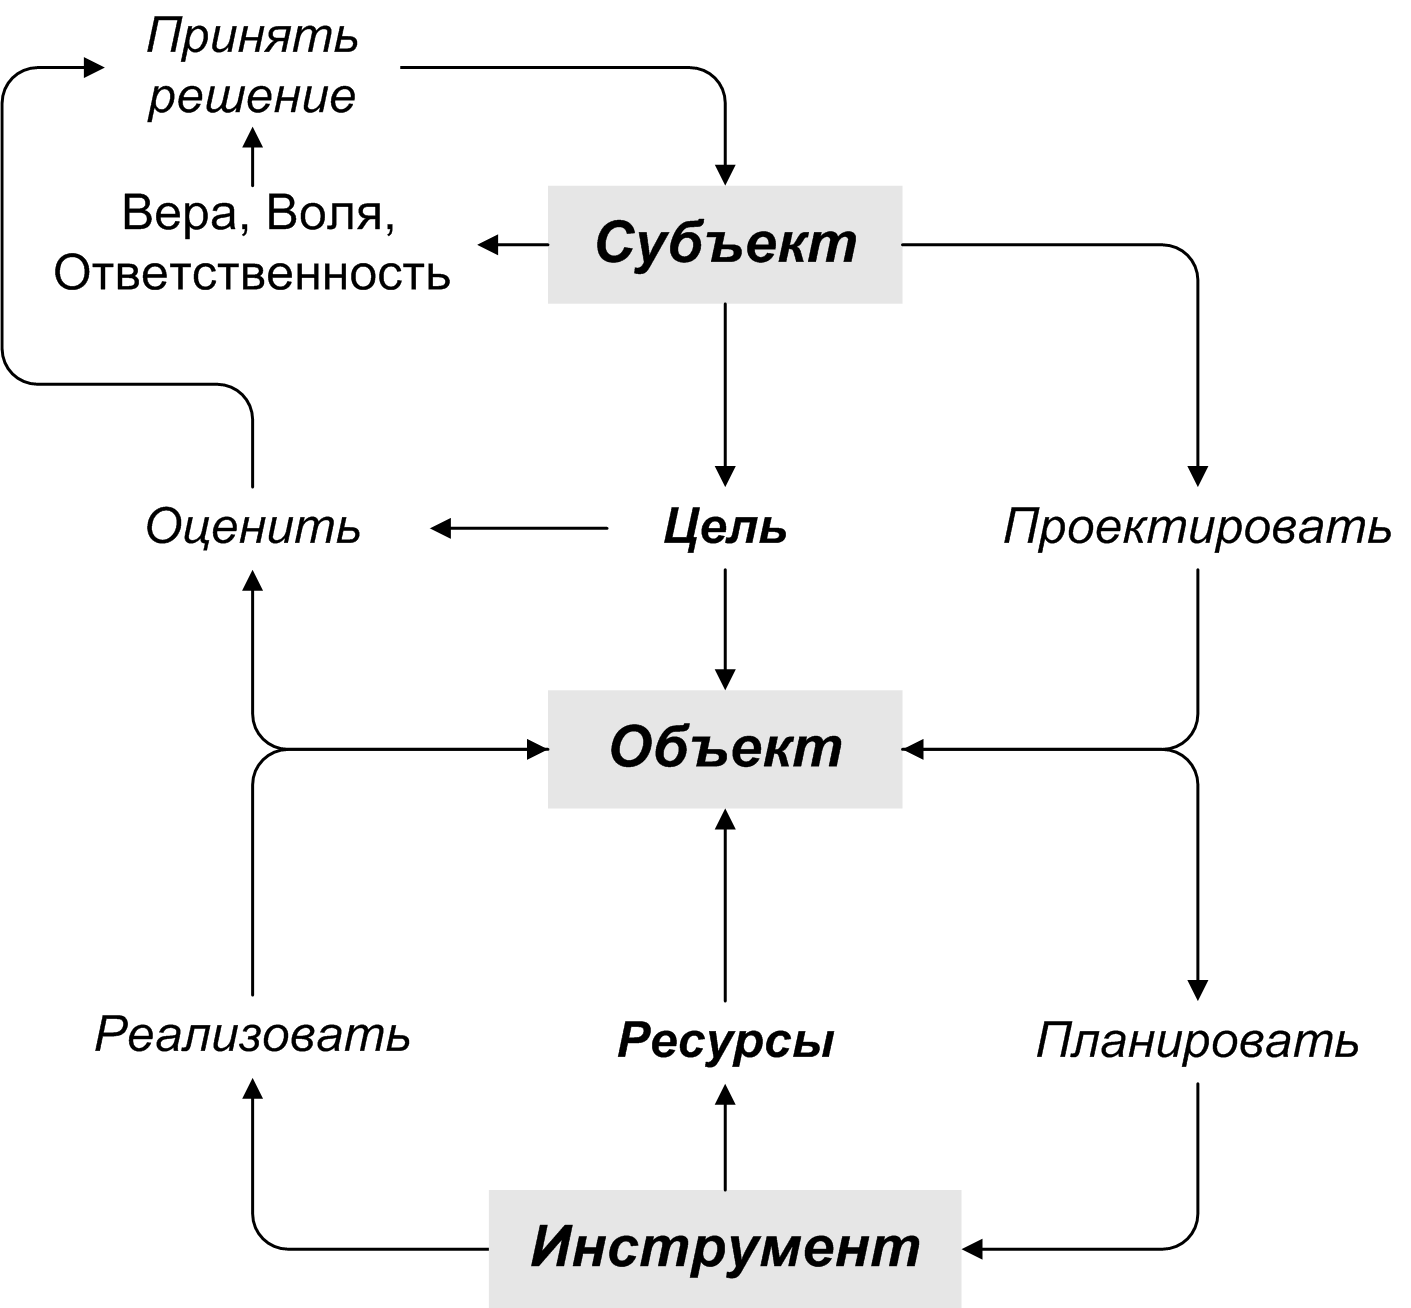
\includegraphics [width=80mm]{pics/mshapb.png}
\caption{Направления взаимодействия субъекта с объектом\label{fig2}}
\end{center}
\end{figure}

%%%%%%%%%%%%%%%%%%%%%%%%%%%%%%%%%%%%%%%%%%%%%%%%%%%%
% Некоторые дополнительные возможности
%
%  \def\propositionname{Предложение}
%  \def\lemmaname{Лемма}
%  \def\assertionname{Утверждение}
%  \def\proofname{Доказательство}
%  \def\corollaryname{Следствие}
%  \def\stagename          {Этап}
%  \def\stepname           {Шаг}
%  \def\algorithmname      {Алгоритм}
%  \def\solutionname       {Решение}
%  \def\axiomname          {Аксиома}
%  \def\ruleofinferencename{Правило вывода}
%  \def\findingsname{Вывод}
%  \def\examplename{Пример}
%  \def\explanationname{Пояснение}
%  \def\notename{Примечание}
%  \def\problemname{Проблема}
%  \def\hypothesisname     {Гипотеза}
%  \def\heuristicsname     {Эвристика}
%  \def\thesisname         {Тезис}
%  \def\taskname           {Задача}
%  \def\rulename           {Правило}
%  \def\wherename{где}
%  \def\listfigurename{Список иллюстраций}
%  \def\listtablename{Список таблиц}
%  \def\subjectindexname{Предметный указатель}
%  \def\alphabeticalindexname{Алфавитный указатель}
%  \def\glossaryname{Глоссарий}
%  \def\thanksname{Благодарности}
%%%%%%%%%%%%%%%%%%%%%%%%%%%%%%%%%%%%%%%%%%%%%%%%%%%%
\subsection{Пояснения}
Если нарушаются границы нижнего колонтитула, то можно произвести принудительный разрыв страницы (\textsf{newpage}).

В комментариях исходного текста упрятаны дополнительные окружения и команды.

\conclusion
Выводы и заключения.

%\begin{thanks}
\thanks
%\begin{acknowlegments}
Автор благодарит коллег и отмечает\ldots

Работа выполнена при финансовой поддержке\ldots%}
%\end{thanks}
%\end{acknowlegments}
\begin{thebibliography}{99}
\bibitem{m1} Автор И.О. Название книги --- М.: Издательство, 2002. --- 700~с.
\bibitem{m2} Автор И.О. Статья // В книге --- Ижевск: Издательство, 2011. --- С.~71-90.
\bibitem{m3} Сайт ТИПД-2014 // \url{http://itpa2014.conf.udsu.ru/}
\end{thebibliography}
%\listoffigures
%\listoftables
\end{document}
